\documentclass[10pt]{beamer}

\usetheme[progressbar=frametitle]{metropolis}
\usepackage{appendixnumberbeamer}

\usepackage{booktabs}
\usepackage[scale=2]{ccicons}

\usepackage{pgfplots}
\usepgfplotslibrary{dateplot}

\usepackage{xspace}
\newcommand{\themename}{\textbf{\textsc{metropolis}}\xspace}

\usepackage{graphicx}

\usepackage{subcaption}

\usepackage[export]{adjustbox}

\title{EE5327 : Optimization}
% \date{\today}
\date{}
\author{Harsh Raj - MA17BTECH11003 \newline Aravind Reddy K V - MA17BTECH11010}
\institute{Mathematics and Computing, IIT-Hyderabad}
% \titlegraphic{\hfill\includegraphics[height=1.5cm]{logo.pdf}}

\begin{document}

\maketitle

\begin{frame}[fragile]{Question}
	Plot the circles 
%
\begin{equation}
\label{eq2_1_circ}
f(\textbf{x}) = (x_1-8)^2 + (x_2-6)^2 = r^2
\end{equation}
%
 $\textbf{x}= (x_1,x_2)^{T}$, for different values of $r$ along with the line 
%
\begin{equation}
\label{eq2_1_line}
g(\textbf{x}) = x_1 + x_2 - 9 = 0
\end{equation} 
%
From the graph, find
\begin{gather*} 
	\min_{\textbf{x}}  f(\textbf{x}) \quad \text{s.t.} \\
	g(\textbf{x}) = x_1 + x_2 - 9 = 0
\end{gather*} 
Also obtain a theoretical solution for the problem above using coordinate geometry.
\end{frame}

\section{Graphical Approach}

\begin{frame}[fragile]{Graphical Approach}
Plotting for different values of r
  \graphicspath{ {./images/} }
  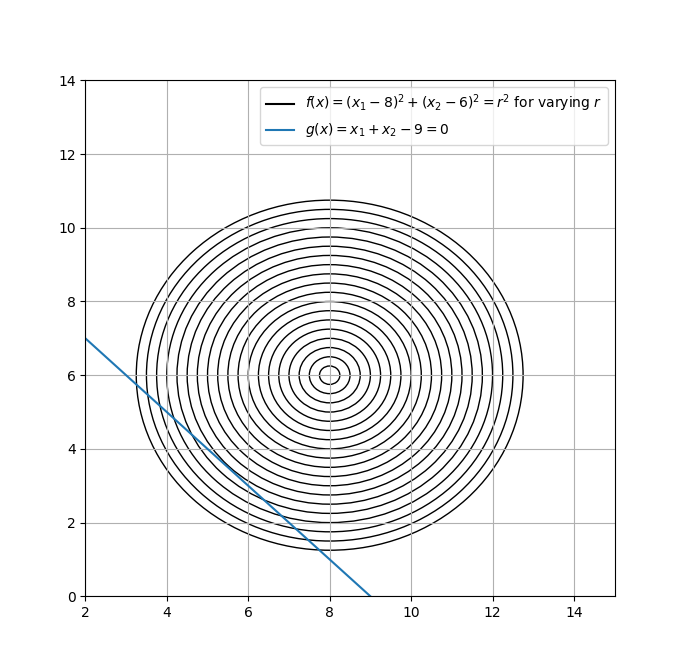
\includegraphics[scale=0.45,center]{Q1}
\end{frame}
{
\metroset{titleformat frame=allsmallcaps}
\begin{frame}{Graphical Approach}
From the graph, find minimum value of $f(\textbf{x})$ satisfying $g(\textbf{x}) = 0$ 
    \graphicspath{ {./images/} }
    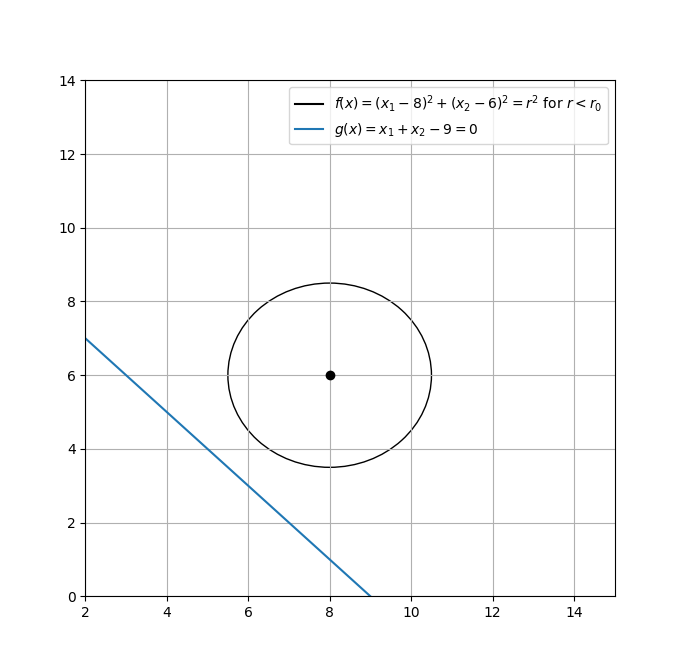
\includegraphics[scale=0.45,center]{2D_1}
\end{frame}
}

{
\metroset{titleformat frame=allsmallcaps}
\begin{frame}{Graphical Approach}
From the graph, find minimum value of $f(\textbf{x})$ satisfying $g(\textbf{x}) = 0$
	\graphicspath{ {./images/} }
    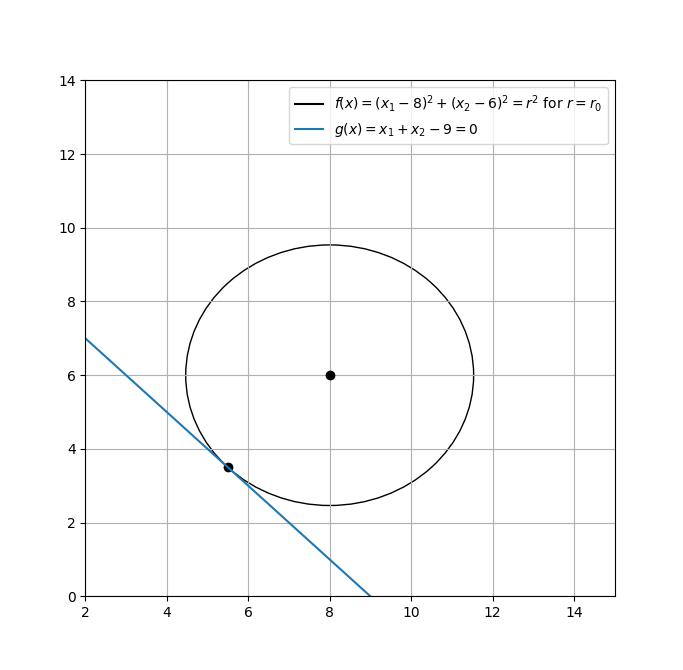
\includegraphics[scale=0.45,center]{2D_2}
\end{frame}
}

{
\metroset{titleformat frame=allsmallcaps}
\begin{frame}{Graphical Approach}
From the graph, find minimum value of $f(\textbf{x})$ satisfying $g(\textbf{x}) = 0$
	\graphicspath{ {./images/} }
    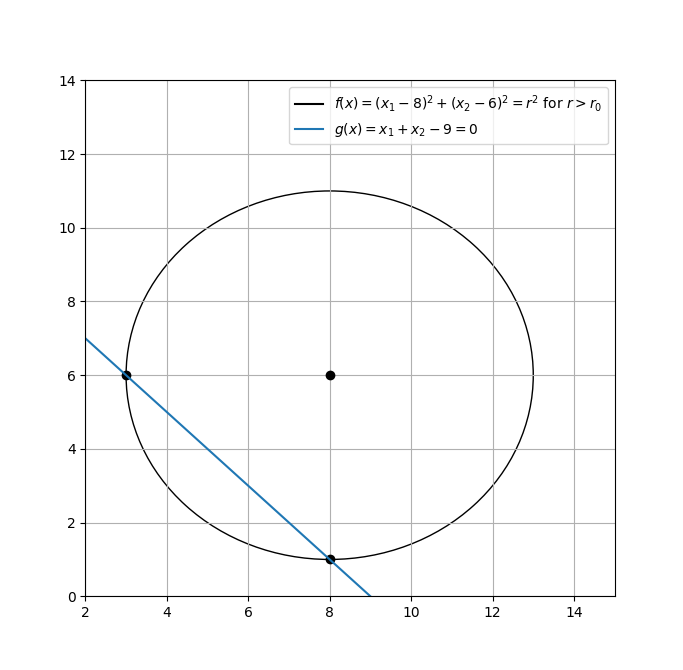
\includegraphics[scale=0.45,center]{2D_3}
\end{frame}
}
{
\metroset{titleformat frame=allsmallcaps}
\begin{frame}{Graphical Approach}


From graph, \newline
%
Since the optimal point lies on the line $g(\textbf{x}) = 0$, it's coordinates satisfy the relation:
\begin{equation}
    x_1+x_2=9
\end{equation}
Using this relation in $f(\textbf{x})$, we get
\begin{align}
r^2 & = (x_1-8)^2 + (3- x_1)^2 \\
&= 2 x_1^2 - 22 x_1 + 73 \\
\Rightarrow r^2 &= \frac{\brak{(2x_1-11)}^2 + 5^2}{2}
\end{align}
%
This is minimum at $x_1 = \frac{11}{2}$.\newline 
To find $x_2$, we use equation (3)  \Rightarrow $x_2 = 9-x_1 =\frac{7}{2}$.  
\newline \newline Hence,    $f(\boldsymbol{x})_{min} = \frac{25}{2}$ at $(\frac{11}{2},\frac{7}{2})$ and $r_{min} = \frac{5}{\sqrt{2}}$. 
\end{frame}
}

\section{Another Graphical Approach}

\begin{frame}{Another Graphical Approach}
Plot Objective z=f(\boldsymbol{x}) and Feasible Region g(\boldsymbol{x})=0.
  \begin{figure}[h]
  \graphicspath{ {./images/} }
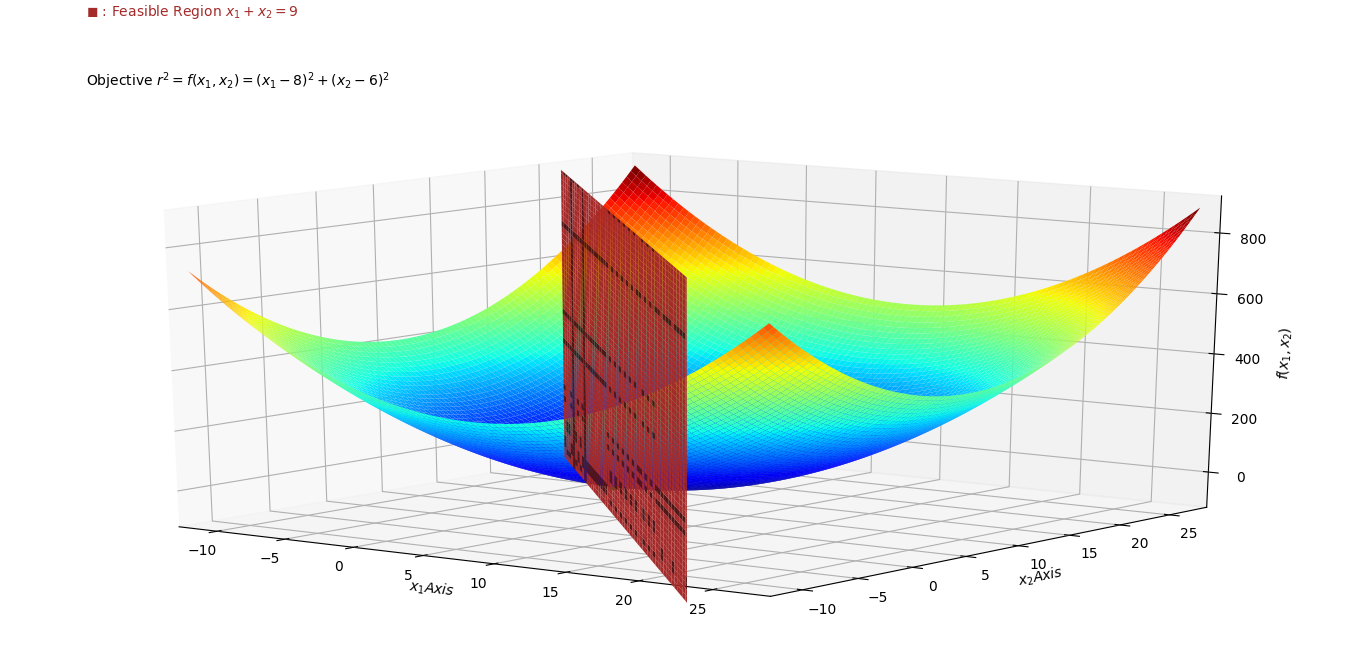
\includegraphics[scale = 0.34]{Figure_1.png}
\end{figure}   
\end{frame}

\begin{frame}{Another Graphical Approach}
From graph, find minimum z=f(\boldsymbol{x}) such that point (\boldsymbol{x},z) lies on feasible region g(\boldsymbol{x})=0.
     \begin{figure}[h]
     \graphicspath{ {./images/} }
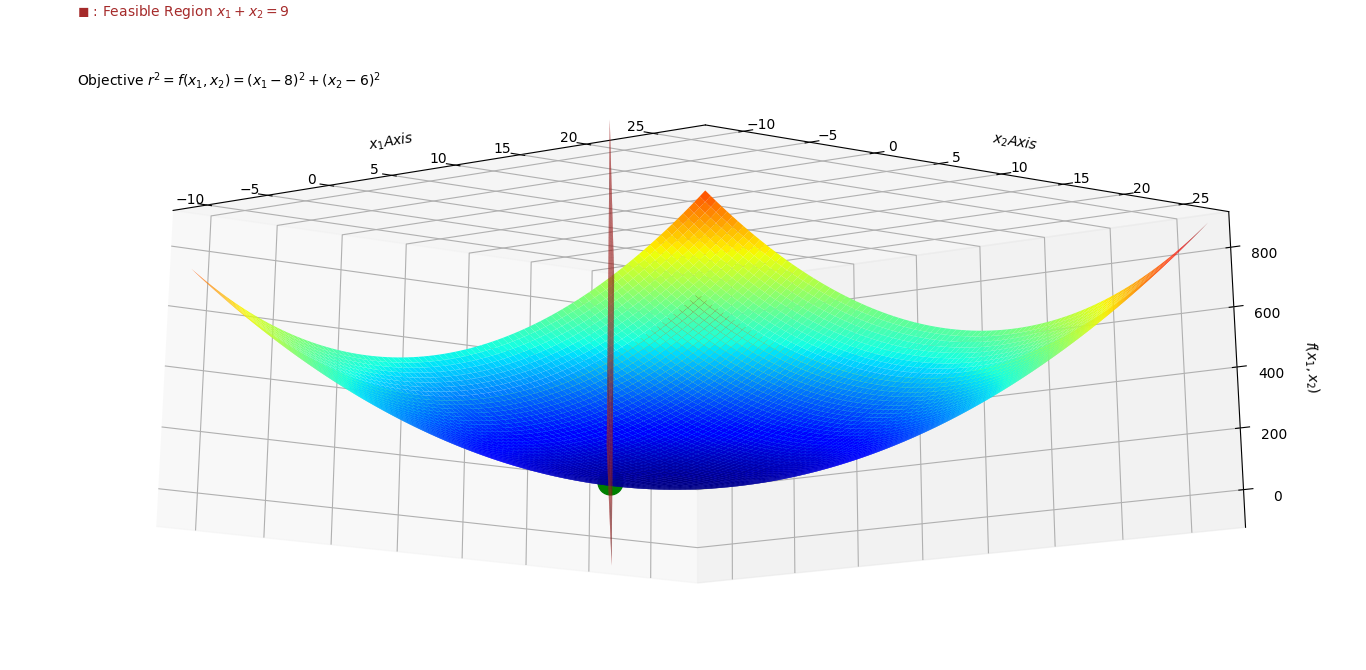
\includegraphics[scale = 0.34]{Figure_2.png}
\end{figure}
\end{frame}

\begin{frame}{Another Graphical Approach}
Finding Constraints for Solving : 
 \begin{figure}[h]
 \graphicspath{ {./images/} }
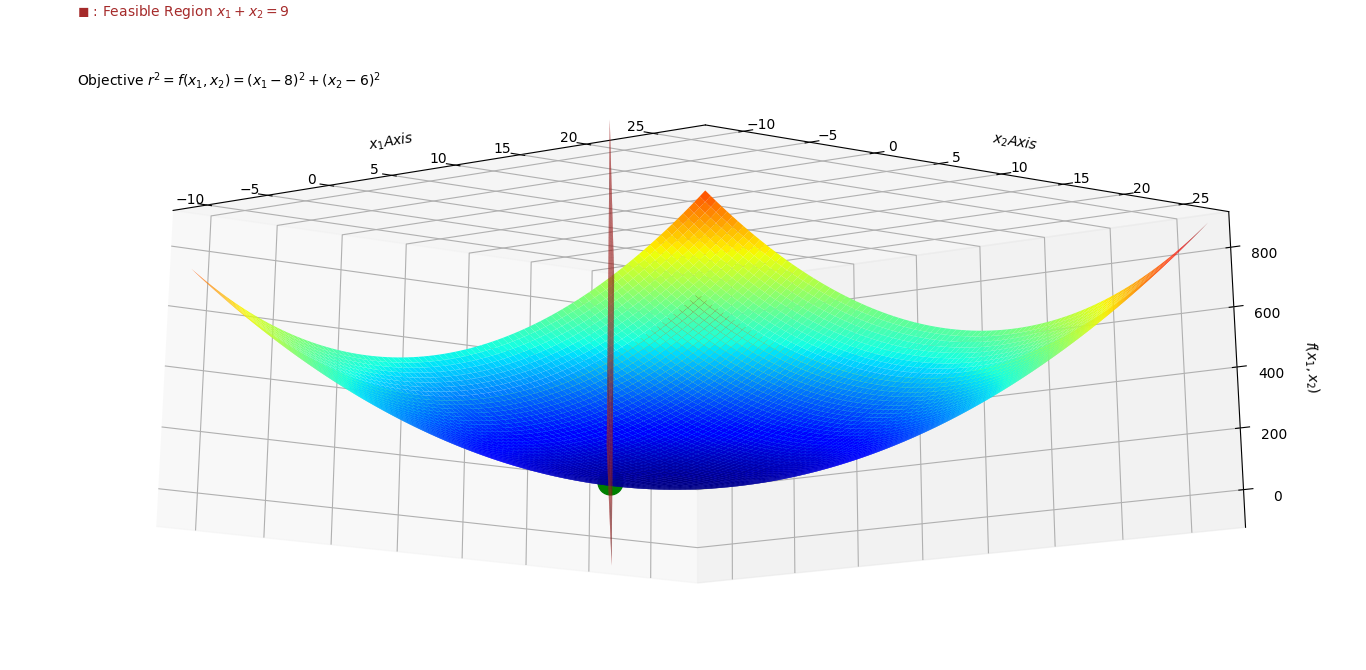
\includegraphics[scale = 0.2]{Figure_2.png}
\end{figure}
As \boldsymbol{x} lies on $g(\boldsymbol{x}) =0 $, \quad \quad $ x_1+x_2=9 $ -(i)
\newline As f(\boldsymbol{x}) is decreasing along $-\nabla$ f(\boldsymbol{x}), and f(\boldsymbol{x}) cannot decrease in any neighbourhood of (\boldsymbol{x},z) in plane, $-\nabla$ f(\boldsymbol{x}) should be perpendicular to plane g(\boldsymbol{x})=0. \quad \quad \quad $-\nabla$ $f(\boldsymbol{x})^T . $\begin{bmatrix}
           9 \\
           -9 \\
          \end{bmatrix}=0-(ii)
          
Solve (i) and (ii) to get $x_1=\frac{11}{2} , x_2=\frac{7}{2} , f(\boldsymbol{x})_{min} = \frac{25}{2}$, $r_{min} = \frac{5}{\sqrt{2}}$
\end{frame}


\end{document}
